\begin{figure}[h]
\caption{Lactose in IQmol}
\label{fig:i2}

\begin{tikzpicture}

\node[inner sep=0pt] (x1) at (0,0)
    {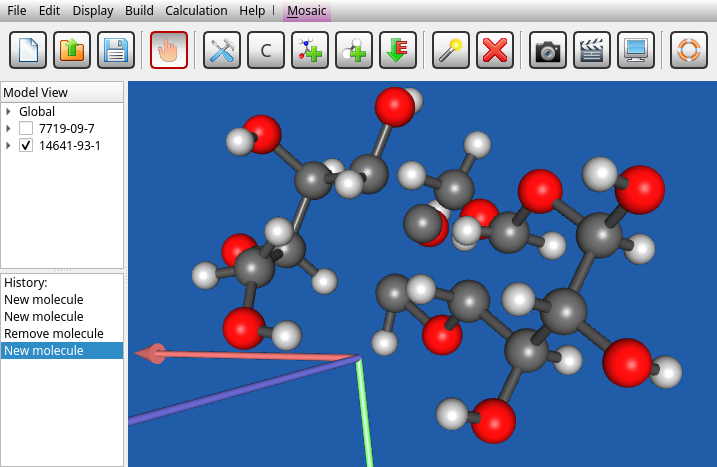
\includegraphics[%width=110mm, 
    	trim={0mm 0 0 0mm},clip]
    	{iScreenShot2.png}};
    \colorlet{cyg}{cyan!70!gray}
 \node [anchor=west,top color=cyg!20,
 bottom color=red!40!brown, shading angle=230, 
 inner sep=3, text width=13.7cm]
 (longnote) at (-9.25,4.8) {\vspace{-8pt}%  %{\color{rb!85!red}{
 {\cframedboxpanda{\vspace{1pt}\large \textbf{%
\makebox{14641-93-1} is the \makebox{Chemical} Abstracts Service 
code for Lactose; 
\makebox{7719-09-7} is the corresponding code 
for Thionyl Chloride.}\vspace{0pt}}}};

\end{tikzpicture}
\end{figure}
